\documentclass{article}

% required includes
\usepackage{graphicx}
\usepackage{url}

\usepackage{tikz}
\usetikzlibrary{shapes,arrows}
% styles for flowcharts
\tikzstyle{machine} = [star, star points=7, star point ratio=0.8, draw, text width=5em, text badly centered, node distance=3cm, inner sep=0pt]
\tikzstyle{data} = [trapezium, trapezium left angle=70, trapezium right angle=-70, draw,text centered]
\tikzstyle{process} = [rectangle, draw, text width=5em, text centered, rounded corners, minimum height=4em] 

\addtolength{\textwidth}{10pt}

\title{CAT-DWAM, A Question Answering System}
\author{
Alec Story,
Ansu Abraham,
Craig Frey,\\
Dustin Tiedemann,
Michael Zhu,
Thomas Levine,
Whitney Foster\\
}

\begin{document}
\maketitle

\section{Overview}

% What are you doing. Why are you doing it.
% ``this is effectively a statement of your hypothesis, so you should
% include justification of why you think that the particular approach
% will be effective

\section{The QA Baseline}
% delete this if you don't think it's necessary
Our baseline system simply takes the first answer of the training data and
repeats that as the answer to all following questions.  It is included as
\verb+zero.py+, and its mean reciprocal rank over 197 questions is 0.048.

\section{The QA System}
% we need:
% a detailed walkthrough of what our system did to handle one question
% (in general) in the corpus. include the system output (enough to
% convince them that it is actually doing what we say)

% this is pretty much the final system proposal from part
% one. delete/rewrite if necessary (we need a description of the
% baseline in our final report)
We implemented our question answering system in Python, and use external
tools such as the natural language toolkit.

Our design mimics the design of Watson, with the intention of trying out a
variety of techniques to select answers from documents, and to use a machine
learning system to choose the appropriate one.  See figure \ref{diagram} for
a graphical overview.

We will first analyze the question (using a parser or hand-written rules) to
determine the parts of speech a valid answer could comprise, so, for example,
``who'' questions always result in a noun phrase, and ``how'' questions usually
result in verb phrases or adverbial phrases.  We will also extract named entities
from the question.

After retrieving the documents, we search for the named entities from the
question in the documents, and return the sentences that match those entities.
These are tagged with their parts of speech, and chunked to produce all the
phrases of the appropriate type determined by analyzing the question.

These are our answer candidates.  They, and their sentence contexts, are passed
into our set of answer evaluators, which associate with them a confidence in
their accuracy.  Simple evaluators include word vector model matching against
the question, and more complex ones might include parsing, or other
sophisticated evaluation techniques.

We will then train a supervised classification algorithm to predict whether
answers are correct based on the confidence measures from the various answer
evaluation techniques. This will produce aggregate confidence measures for
each answer. Finally, we will pack the most confident answers into the 50 bytes
until we run out of space.

\begin{figure}
 \label{diagram}
 \begin{center}
  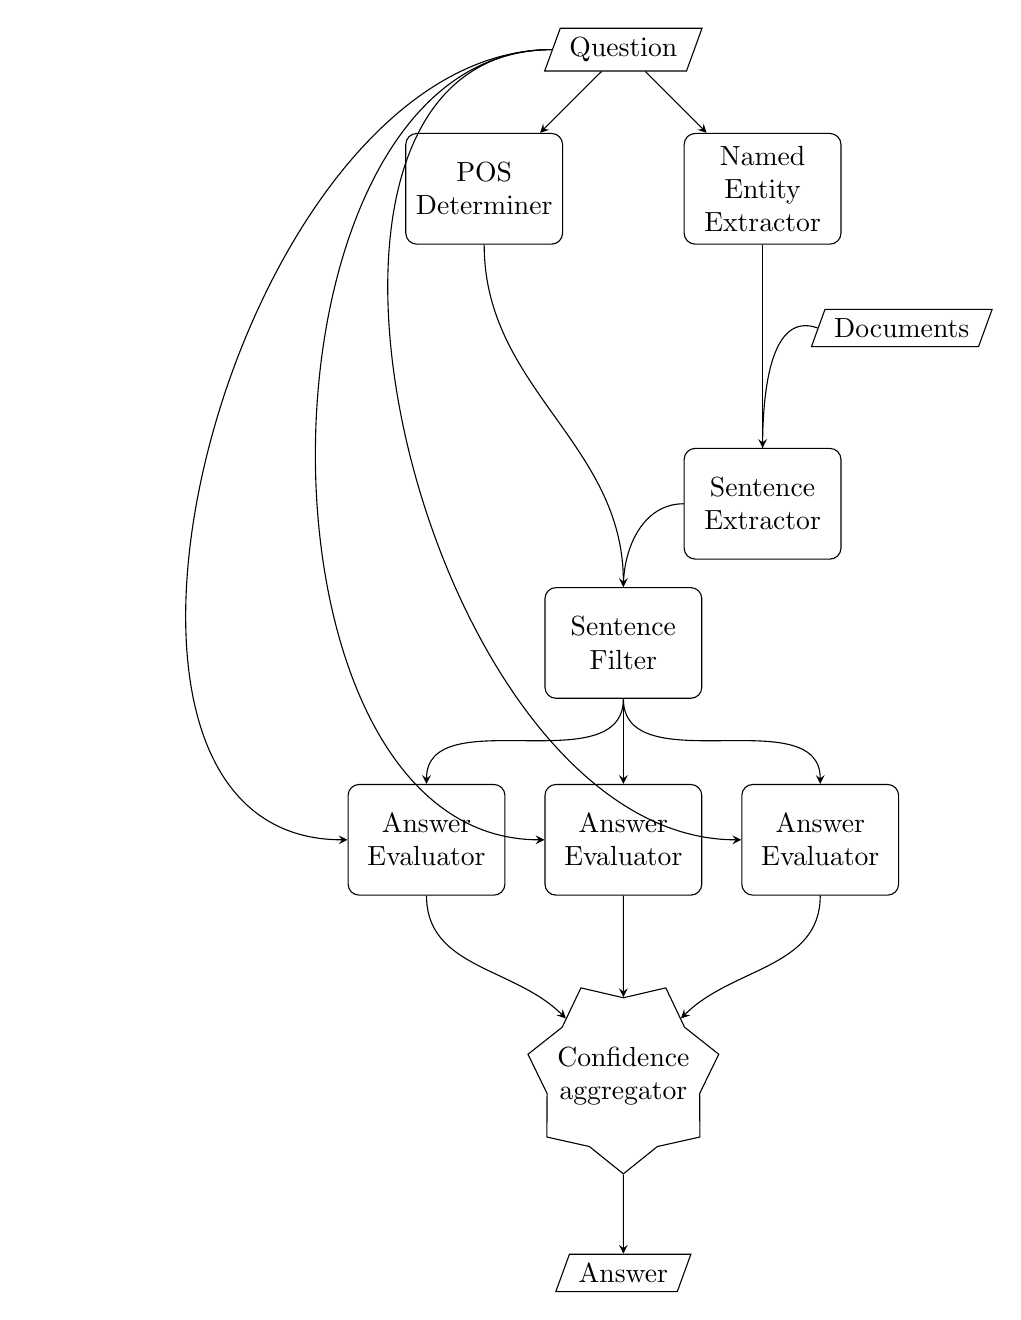
\begin{tikzpicture}[node distance=2.5cm, auto, >=stealth]
   % nodes
   \node[data] (Q)                                      {Question};
   \node[process] (pd) [below left of=Q]                {POS Determiner};
   \node[process] (na) [below right of=Q]               {Named Entity Extractor};
   \node[data] (docs) [below right of=na]               {Documents};
   \node[process] (ex) [below of=na, node distance=4cm] {Sentence Extractor};
   \node[process] (sf) [below left of=ex]               {Sentence Filter};
   \node[process] (a2) [below of=sf]                    {Answer Evaluator};
   \node[process] (a1) [left of=a2]                     {Answer Evaluator};
   \node[process] (a3) [right of=a2]                    {Answer Evaluator};
   \node[machine] (as) [below of=a2]                    {Confidence aggregator};
   \node[data] (A) [below of=as]                        {Answer};
   
   % edges
   	\draw[->] (Q) to (pd);
   	\draw[->] (Q) to (na);
   	\draw[->] (na) to (ex);
	\draw (docs.west) to [out=160, in=90] (ex);
	\draw[->] (pd.south) to [out=270, in=90] (sf);
	\draw (ex.west) to [out=180, in=90] (sf);
	\draw[->] (sf.south) to [out=270, in=90] (a1);
	\draw[->] (sf.south) to [out=270, in=90] (a2);
	\draw[->] (sf.south) to [out=270, in=90] (a3);
	\draw[->] (Q.west) to [out=180, in=180] (a1);
	\draw[->] (Q.west) to [out=180, in=180] (a2);
	\draw[->] (Q.west) to [out=180, in=180] (a3);
	\draw[->] (a1.south) to [out=270, in=135] (as);
	\draw[->] (a2.south) to [out=270, in=90] (as);
	\draw[->] (a3.south) to [out=270, in=45] (as);
	\draw[->] (as) to (A);
  \end{tikzpicture}
  \caption{Data Flow}
  \label{flowchart}
 \end{center}
\end{figure}

\subsection{Parsing the Corpus Documents}
% Talk about Whitney's Shredder module here?

\subsection{The Classifier}

\subsection{Question Evaluators}

\subsubsection{Question-Document Comparison}

	We implemented a system to compare the question and answer against the
	proposed document in two ways:  one, with a na\"ive diffing algorithm that
	simply seeks out the longest indentical sequence, and one by implementing
	the Smith-Waterman local alignment
	algorithm.\footnote{\url{http://en.wikipedia.org/wiki/Smith-Waterman_algorithm}}
	We also implemented a system to attempt to re-write questions, discussed
	below, and applied these same techniques to the re-written question

	The na\"ive method does an adequate job when the document highly resembles
	the question, but does very poorly otherwise because it has no tolerance of
	faults.  The local alignment does much better for documents that resemble
	the question a great deal, but are not precise - it can smoothly deal with
	small differences, and still produce a good alignment.  This is a standard
	technique from bioinformatics, and is used extensively to align small
	sequences of DNA, RNA or protein against a larger corpus, such as a
	chromosome or a whole genome.  This is a fairly similar usage to aligning a
	question against a document which is much longer than the question.

	We chose Smith-Waterman over the similar Needleman-Wunsch, of which is a
	special case, because Needleman-Wunsch creates a \emph{global} alignment,
	which forces all of the characters in both strings to align.  This leads to
	the insertion of many gaps, and needlessly aligns words which are useless,
	for example, ``Who is Queen of England?'' should align well against
	``Elizabeth is Queen of England'' and it does, under Smith-Waterman, but the
	``who'' causes Needleman-Wunsch to choke.  Similarly, Needleman-Wunsch does
	not excuse one string for being shorter than the other, and chokes on all of
	the apparent gaps that it needs to insert, so it is not a good choice.

	We locate what we best believe to be the question via these two methods, and
	then evaluate how far away from that segment of the document the answer is.
	If it is fairly close, that is a good indicator that it is highly related to
	the question, but if it is far, it is likely to be unrelated.  We feed that
	distance, and either the length of the na\"ive alignment or the score that
	Smith-Waterman produces (higher is better for both) because very short or
	very poor alignments are less likely to reflect an actual representation of
	the question.

\subsubsection{Punctuation Filter}
% Ansu

\subsubsection{Apposition Filter}
% Ansu

\subsubsection{Preceding and Proceeding N-grams Filter}
% Tom

\subsubsection{Number and Quantity Answer Type Filters}
% Tom

\subsubsection{Measurement Units or Matching Type Filters}
% Tom

\subsubsection{Sequence Length}
% Mike

\subsubsection{Word Vector (Feature?)}
% Dustin

\subsubsection{Bag of Words Filter}
% Dustin

\subsubsection{Novelty Factor}
% Dustin

\subsubsection{Part of Speech Matching}
% Craig

\subsection{Confidence Measures}

\section{Results}

% we need:
% the output file of answers produced by our system for the questions
% from the development corpus
% an evaluation using the Mean Reciprocal Rank Evaulation Measure)
% an analysis of the system's performance on questions of the
% development corpus
   % what worked?
   % what didn't work?
   % which component was strongest/weakest?
   % how does our system compare to the baseline?
% responses from our system for test set released on Wednesday
   % we also need to submit this file

\subsection{Baseline Results}

\subsection{Graphical Methods}

\subsection{Best Run Results}

\section{Conclusion}

\end{document}
